% 导言区：格式定义（完全匹配模板，无需修改）
\documentclass[12pt,a4paper]{article} % 12号字，A4纸，英文报告基础文档类
\usepackage{geometry} % 页面布局，页边距适配模板
\geometry{left=2.5cm, right=2.5cm, top=2.5cm, bottom=2.5cm}
\usepackage{graphicx} % 插入图片必备
\usepackage{float} % 固定图片/表格位置（防止乱跑）
\usepackage{booktabs} % 美化表格（可选，匹配模板简约风格）
\usepackage{amsmath} % 公式支持（若需要加公式可保留）
\renewcommand{\baselinestretch}{1.15} % 行间距，适配PDF阅读体验

% 标题、作者、日期
\title{\bfseries \Large Report of Regression and Non-linear Deep Learning Models} 
\author{Li Chao\\ 
superlee0183@gmail.com} 
\date{\today} 

\begin{document}
\maketitle 


\begin{abstract}
This report presents a comparative study on various optimization algorithms for linear regression, including Least Squares, Gradient Descent, and Newton's Method. Based on the observation of underfitting caused by the non-linear nature of the provided dataset, a Multi-Layer Perceptron (MLP) model is further proposed and evaluated. The results demonstrate that deep learning approaches significantly minimize both training and testing errors by capturing complex non-linear mappings.
\end{abstract}

\section{Introduction}
Regression analysis is a fundamental technique in machine learning used to model the relationship between a dependent variable and one or more independent variables. In this study, we are given a 2-dimensional dataset comprising separate training and test sets. 

The primary objective of this report is to first fit a linear model to the data using three classic optimization techniques. Furthermore, recognizing the inherent limitations of linear models on non-linear data distributions, we propose replacing the linear approach with a non-linear neural network model to improve the fitting performance.

\section{Proposed Methods}

\subsection{Linear Models Optimization}
To establish a baseline, we employ three different optimization methods to train a linear model $y = wx + b$:
\begin{itemize}
    \item \textbf{Least Squares (LS):} Directly computes the global optimum using the closed-form analytical solution $w = (X^T X)^{-1} X^T y$.
    \item \textbf{Gradient Descent (GD):} An iterative optimization algorithm that updates the weights by taking steps proportional to the negative gradient of the Mean Squared Error (MSE) loss function.
    \item \textbf{Newton's Method:} Utilizes both the first-order gradient and the second-order Hessian matrix. For linear regression, Newton's method optimally converges in a single iteration.
\end{itemize}

\subsection{Non-linear MLP Model}
Because the provided dataset exhibits significant non-linearity, forcing a linear model results in severe underfitting. To address this, we introduce a \textbf{Multi-Layer Perceptron (MLP)}. \\
The MLP features hidden layers coupled with ReLU activation functions, granting it the universal approximation capability. This enables the model to effectively map the complex, non-linear curvature of the data, substantially enhancing both model accuracy and generalization.

\section{Experimental Studies}
In our experiments, the linear optimization methods uniformly converged to the exact same fitting line, yielding identically high Mean Squared Errors (MSE). Subsequently, the MLP model (configured with 2 hidden layers of 100 neurons each) was applied.

Table \ref{tab:1} outlines the comparative training and testing errors. The results evidently show that the MLP model drastically reduced the MSE compared to linear methods.

\begin{table}[H] 
    \centering 
    \caption{MSE Comparison of Different Models} 
    \begin{tabular}{lcc} 
        \toprule 
        \textbf{Model / Method} & \textbf{Training MSE} & \textbf{Test MSE} \\
        \midrule 
        Least Squares & 0.6134 & 0.5950 \\
        Gradient Descent & 0.6134 & 0.5947 \\
        Newton's Method & 0.6134 & 0.5950 \\
        \textbf{MLP Regressor} & \textbf{0.3826} & \textbf{0.4227} \\
        \bottomrule 
    \end{tabular}
    \label{tab:1} 
\end{table}

Figure \ref{fig:1} visually contrasts the fitting performances. The left plot demonstrates the linear model's rigidity (underfitting), whereas the right plot showcases the MLP's ability to smoothly follow the dataset's non-linear trend.

\begin{figure}[H] 
    \centering 
    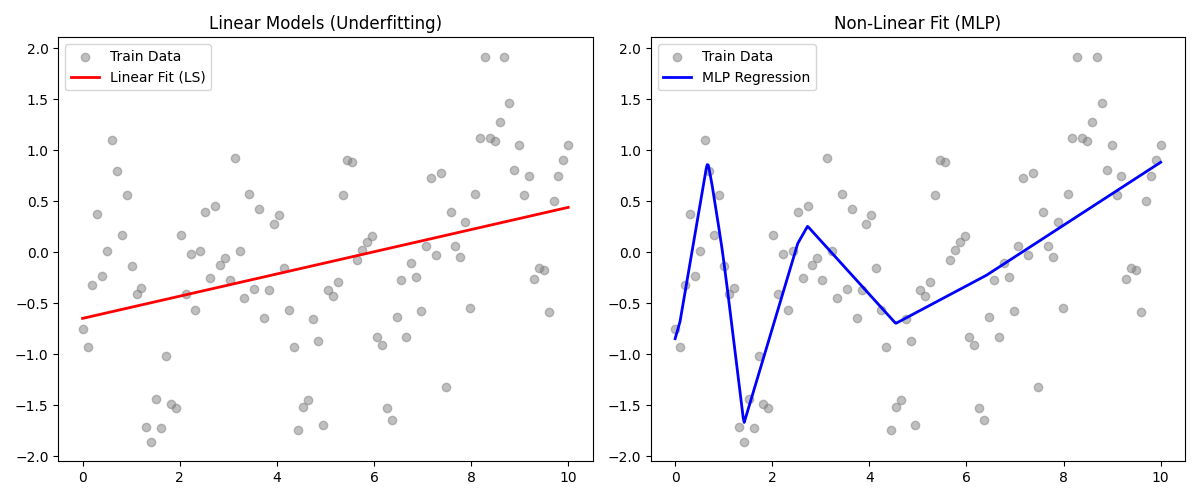
\includegraphics[width=0.9\textwidth]{fit_results.png} % 请确保 Python 保存的图片在此路径下
    \caption{Comparison of Linear Fitting vs. Non-linear MLP Fitting}
    \label{fig:1}
\end{figure}

\end{document}